\documentclass[a4paper,12pt]{article} % добавить leqno в [] для нумерации слева
\usepackage[a4paper,top=1.3cm,bottom=2cm,left=1.5cm,right=1.5cm,marginparwidth=0.75cm]{geometry}
%%% Работа с русским языком
\usepackage{cmap}					% поиск в PDF
\usepackage{mathtext} 				% русские буквы в фомулах
\usepackage[T2A]{fontenc}			% кодировка
\usepackage[utf8]{inputenc}			% кодировка исходного текста
\usepackage[english,russian]{babel}	% локализация и переносы

\usepackage{graphicx}

\usepackage{wrapfig}
\usepackage{tabularx}

\usepackage{hyperref}
\usepackage[rgb]{xcolor}
\hypersetup{
colorlinks=true,urlcolor=blue
}
\usepackage{multirow}
\usepackage{hhline}


%%% Дополнительная работа с математикой
\usepackage{amsmath,amsfonts,amssymb,amsthm,mathtools} % AMS
\usepackage{icomma} % "Умная" запятая: $0,2$ --- число, $0, 2$ --- перечисление

%% Номера формул
\mathtoolsset{showonlyrefs=true} % Показывать номера только у тех формул, на которые есть \eqref{} в тексте.

%% Шрифты
\usepackage{euscript}	 % Шрифт Евклид
\usepackage{mathrsfs} % Красивый матшрифт

%% Свои команды
\DeclareMathOperator{\sgn}{\mathop{sgn}}

%% Перенос знаков в формулах (по Львовскому)
\newcommand*{\hm}[1]{#1\nobreak\discretionary{}
{\hbox{$\mathsurround=0pt #1$}}{}}

\begin{document}

\newenvironment{lines}[1][\textwidth] % по умолчанию линейки на всю ширину текста
{
\newcolumntype{E}{>{}p{#1}<{\hrulefill}} % в конце нашего столбца будет приписываться \hrulefill
\begin{flushright} % автоматически вставим flushright
\begin{tabular}[h]{E} % и tabular нужного формата
}
{\end{tabular}\end{flushright}
}
	
	\begin{titlepage}
	\begin{center}
		{\large МОСКОВСКИЙ ФИЗИКО-ТЕХНИЧЕСКИЙ ИНСТИТУТ (НАЦИОНАЛЬНЫЙ ИССЛЕДОВАТЕЛЬСКИЙ УНИВЕРСИТЕТ)}
	\end{center}
	\begin{center}
		{\large Физтех-школа электроники, фотоники и молекулярной физики}
	\end{center}
	
	
	\vspace{4.5cm}
	{\huge
		\begin{center}
			{Лабораторная работа 5.1.2}\\
			Исследование эффекта Комптона
		\end{center}
	}
	\vspace{2cm}
	\begin{flushright}
		{\LARGE Салтыкова Дарья \\
			\vspace{0.5cm}
			Б04-105}
	\end{flushright}
	
	\vspace{0.5cm}
	
	\begin{lines}[.5
	\textwidth]
  {\LARGE Допуск} \rule{6.5cm}{0.25pt} \vspace{0.5cm}\\
 {\LARGE Выполнение} \rule{3cm}{0.25pt}\vspace{0.5cm} \\ {\LARGE Сдача} \rule{3cm}{0.25pt} \\ % \rule сделает линейку указанной длины и толщины
\end{lines}
	\vspace{8cm}
	\begin{center}
		Долгопрудный 2023
	\end{center}
\end{titlepage}

\section{Введение}

\noindent
\textbf{Цель работы:} Исследование энергетического спектра $\gamma$-квантов, рассеянных на графите, с помощью сцинтилляционного спектрометра. Определение энергии рассеянных $\gamma$-квантов в зависимости от угла рассеяния. Определение энергии покоя частиц, на которых происходит комптоновское рассеяние.
\medskip

\noindent \textbf{В работе используются:} источник излучения, графитовая мишень, сцинтилляционный счётчик, ФЭУ, ЭВМ.

\medskip

\section{Теоретические сведения}
\noindent \textbf{Эффект Комптона} - увеличение длины волны рассеянного излучения по сравнению с падающим. Он интерпретируется как результат упругого соударения двух частиц - $\gamma$-кванта и свободного электрона.

 \medskip

\noindent Пусть электрон до соударения покоился, а  $\gamma$-квант имел начальную энергию \hbar$\omega_0$ и импульс \hbar$\omega_0/c$. После соударения электрон приобретает энергию $\gamma mc^2$, где $\gamma = (1 − \beta^2)^{−1/2}$, $\beta = v/c$, а  $\gamma$-квант рассеивается на некоторый угол $\theta$ по отношению
к первоначальному направлению движения. Энергия и импульс рассеянного излучения — $\propto \omega_1$. Запишем для рассматриваемого процесса законы сохранения энергии и импульса:

\begin{center}
    $mc^2 +$ $\hbar \omega_0 = \gamma mc^2 +$ $\hbar \omega_1$\\
    $\frac{\hbar \omega_0}{c} = \gamma mv \cos \varphi + \frac{\hbar \omega_1}{c} \cos \theta$ \\
    $\gamma mv \sin \varphi = \frac{\hbar \omega_1}{c} \sin \theta$
\end{center}

\noindent Решая совместно эти уравнения и переходя от частот к длинам волн, получаем изменение длины рассеянного излучения

\begin{equation}
    \triangle \lambda = \lambda_1 - \lambda_0 = \frac{h}{mc}(1 - \cos \theta) = \Lambda_k(1 - \cos \theta),
\end{equation}

\noindent где $\Lambda_k = \frac{h}{mc} = 2.42 \dot 10^{-10}$ см - комптоновская длина волны электрона.

 \medskip

\noindent Основной целью работы является проверка соотношения (1). Преобразуем его от длин волн к энергии $\gamma$-квантов:

\begin{equation}
    \frac{1}{\varepsilon(\theta)} - \frac{1}{\varepsilon_0} = 1 - \cos \theta,
\end{equation}

\noindent где $\varepsilon_0 = E_0/(mc^2)$ - энергия $\gamma$-квантов, падающих на рассеиватель (в единицах $mc^2$), $\varepsilon(\theta)$ - выраженная в тех же единицах энергия квантов, испытавших комптоновское рассеяния на угол $\theta$, $m$ - масса электрона.

\newpage

\section{Экспериментальная установка}

  \begin{figure}[h!]
\begin{center}
\begin{minipage}[h!]{0.48\linewidth}
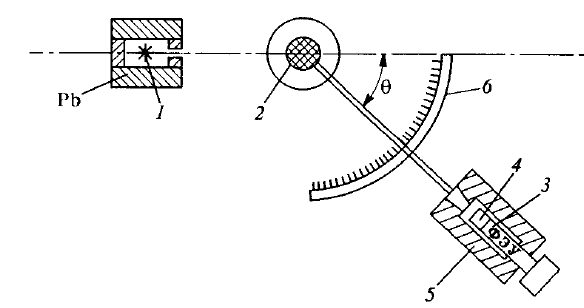
\includegraphics[width=1\linewidth]{fig2.PNG}
\caption{Блок-схема установки по изучению рассеяния $\gamma$-квантов} %% подпись к рисунку\label{ris:experimoriginal} %% метка рисунка для ссылки на него
\end{minipage}
\hfill 
\begin{minipage}[h!]{0.48\linewidth}
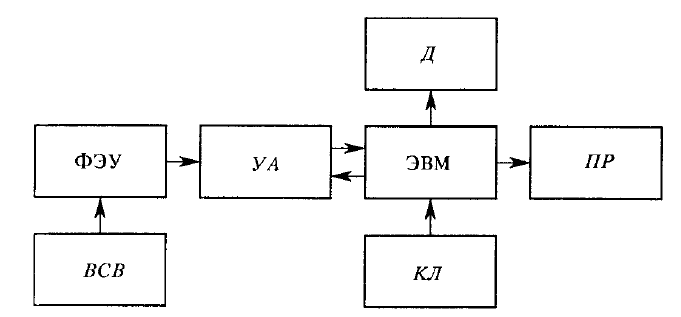
\includegraphics[width=1\linewidth]{fig3.PNG}
\caption{Блок-схема измерительного комплекса}
\label{ris:experimcoded}
\end{minipage}
\end{center}
\end{figure}

\noindent Источником излучения служит $^{137}$Cs(1), испускающий  $\gamma$-кванты с энергией 662 кэВ. Узкий пучок после коллиматора попадает на графитовую мишень (2). Кванты, испытавшие комптоновское рассеяния в мишени, регистрируются сцинтилляционным счетчиком и проходят на ФЭУ. Сигналы, возникающие на ФЭУ, подаются на ЭВМ для амплитудного анализа. Штанга с измерительным блоком может вращаться относительно мишени.

\section{Ход работы}

\noindent 1. Проверим, что при увеличении угла фотопик смещается влево.

\medskip

\noindent 2. Устанавливая сцинтилляционный датчик под разными углами,получаем картины пиков, по которым измеряем номера каналов. Полученные данные занесем в таблицу.

\medskip

\begin{table}[h!]
\begin{tabular}{|l|l|l|l|}
\hline
$\text{Угол},  ^\circ$ & Канал & $1 - cos(\theta)$ & $1/N(\theta)$ \\ \hline
0                      & 804   & 0                 & 0,001244      \\ \hline
10                     & 856   & 0,01519           & 0,001168      \\ \hline
20                     & 757   & 0,06031           & 0,001321      \\ \hline
30                     & 697   & 0,13397           & 0,001435      \\ \hline
40                     & 639   & 0,23396           & 0,001565      \\ \hline
50                     & 575   & 0,35721           & 0,001739      \\ \hline
60                     & 510   & 0,50000           & 0,001961      \\ \hline
70                     & 448   & 0,65798           & 0,002232      \\ \hline
80                     & 401   & 0,82635           & 0,002494      \\ \hline
90                     & 368   & 1                 & 0,002717      \\ \hline
100                    & 336   & 1,17365           & 0,002976      \\ \hline
110                    & 314   & 1,34202           & 0,003185      \\ \hline
120                    & 293   & 1,50000           & 0,003413      \\ \hline
\end{tabular}
\end{table}

\medskip

\noindent Заметим, что для более точного анализа погрешностей следовало бы сохранять первоначальные данные полностью, но программное обеспечение не позволяет это делать. Оцифровка была сделана для $\theta = 0 ^\circ$ с нашими данными и для некоторых других углов с данными коллег (см. ниже).

\medskip

\noindent 3. Перейдем к проверке соотношения $\frac{1}{N(\theta)} - \frac{1}{N(0)} = A(1 - cos \theta).$ Построим график зависимости $\frac{1}{N(\theta)} - \frac{1}{N(0)}(1 - cos \theta)$.

\begin{figure}[h!]
    \centering
    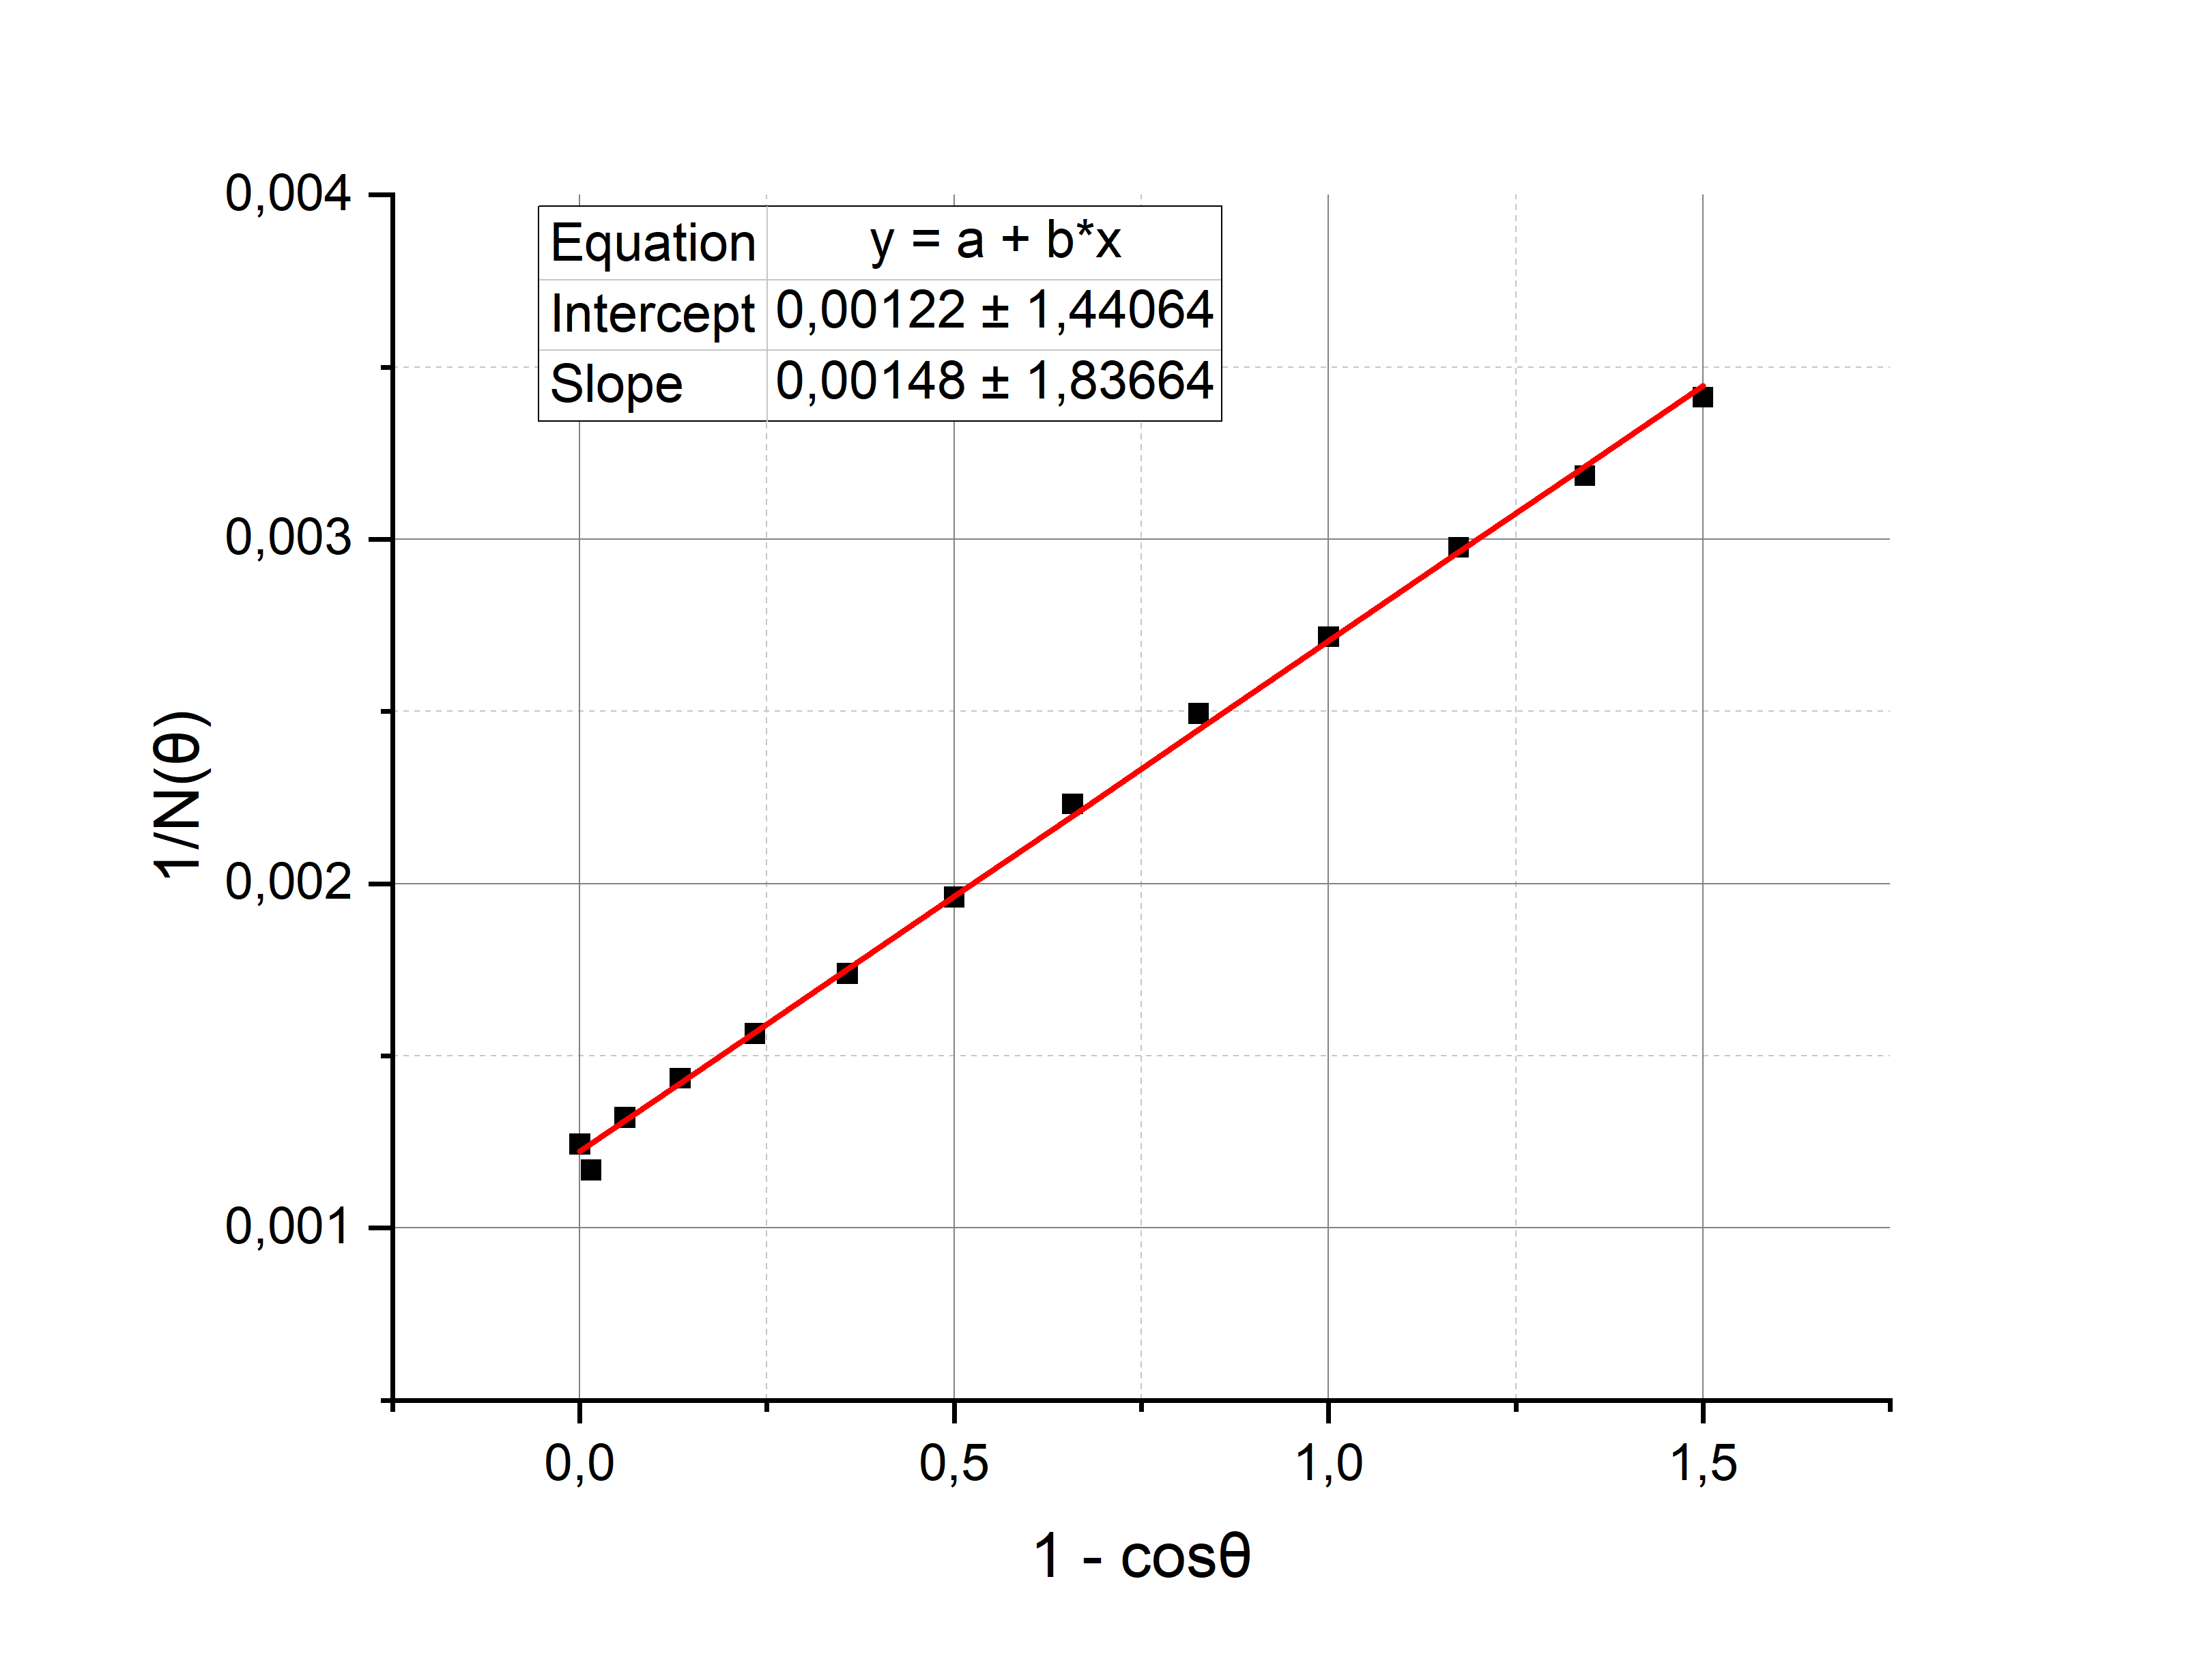
\includegraphics[scale=0.5]{гр.png}
    \caption{Зависимость $\frac{1}{N(\theta)} - \frac{1}{N(0)}(1 - cos \theta)$}
\end{figure}

\noindent 4. Рассчитаем энергию покоя частицы, на которой происходит комптоновское рассеяние.

\medskip

\noindent Из графика: $N_\text{наил}(0 ^\circ) = 819 \pm 13, \frac{1}{N_\text{наил}(90 ^\circ)} = (270 \pm 4) \cdot 10^{-5}, N_\text{наил}(90 ^\circ) = 370 \pm 6.$

$$mc^2 = E_{\gamma} \frac{N_\text{наил}(90 ^\circ)}{N_\text{наил}(0^\circ)-N(_\text{наил}90^\circ)} = 545 \pm 17 \text{ кэВ}.$$

\noindent Погрешность складывается из погрешностей определения угла и погрешности опредления положения пика.

\section{Оценка погрешностей}

\noindent Оцифруем получившиеся графики, аппроксимируем фотопики по Гауссу и определим точное положение пиков. Сравним полученные таким образом значения с теми, что были полчены в ходе эксперимента. Оцифрованные графики см. в Приложении.

\begin{table}[h!]
\begin{tabular}{|l|l|l|l|l|l|}
\hline
$\text{Угол},   ^\circ$ & 0   & 20  & 50  & 60  & 90  \\ \hline
Грубо                   & 804 & 771 & 542 & 486 & 338 \\ \hline
Точно                   & 806 & 766 & 546 & 480 & 341 \\ \hline
\end{tabular}
\end{table}

\noindent Как видим, грубая оценка в среднем отличается от точной на $0,75\%$.

\section{Вывод}

\noindent В работе был исследован эффект Комптона на графите с помощью сцинтилляционного спектрометра. При этом была выяснена зависимость энергии рассеянного $\gamma-$кванта от угла рассеяния, а также определена величина энергии покоя электрона $mc^2 = 545 \pm 17 \text{ кэВ}.$ Теоретическое значение $(mc^2)_\text{теор} = 511 \text{ кэВ}.$ Разницу в значениях можно объяснить тем, что в нашем эксперименте расчетная формула недостаточно точна, ввиду того что электронs в составе атомов исследуемого вещества не являются свободными.

\section{Приложение}

\begin{figure}[h!]
    \centering
    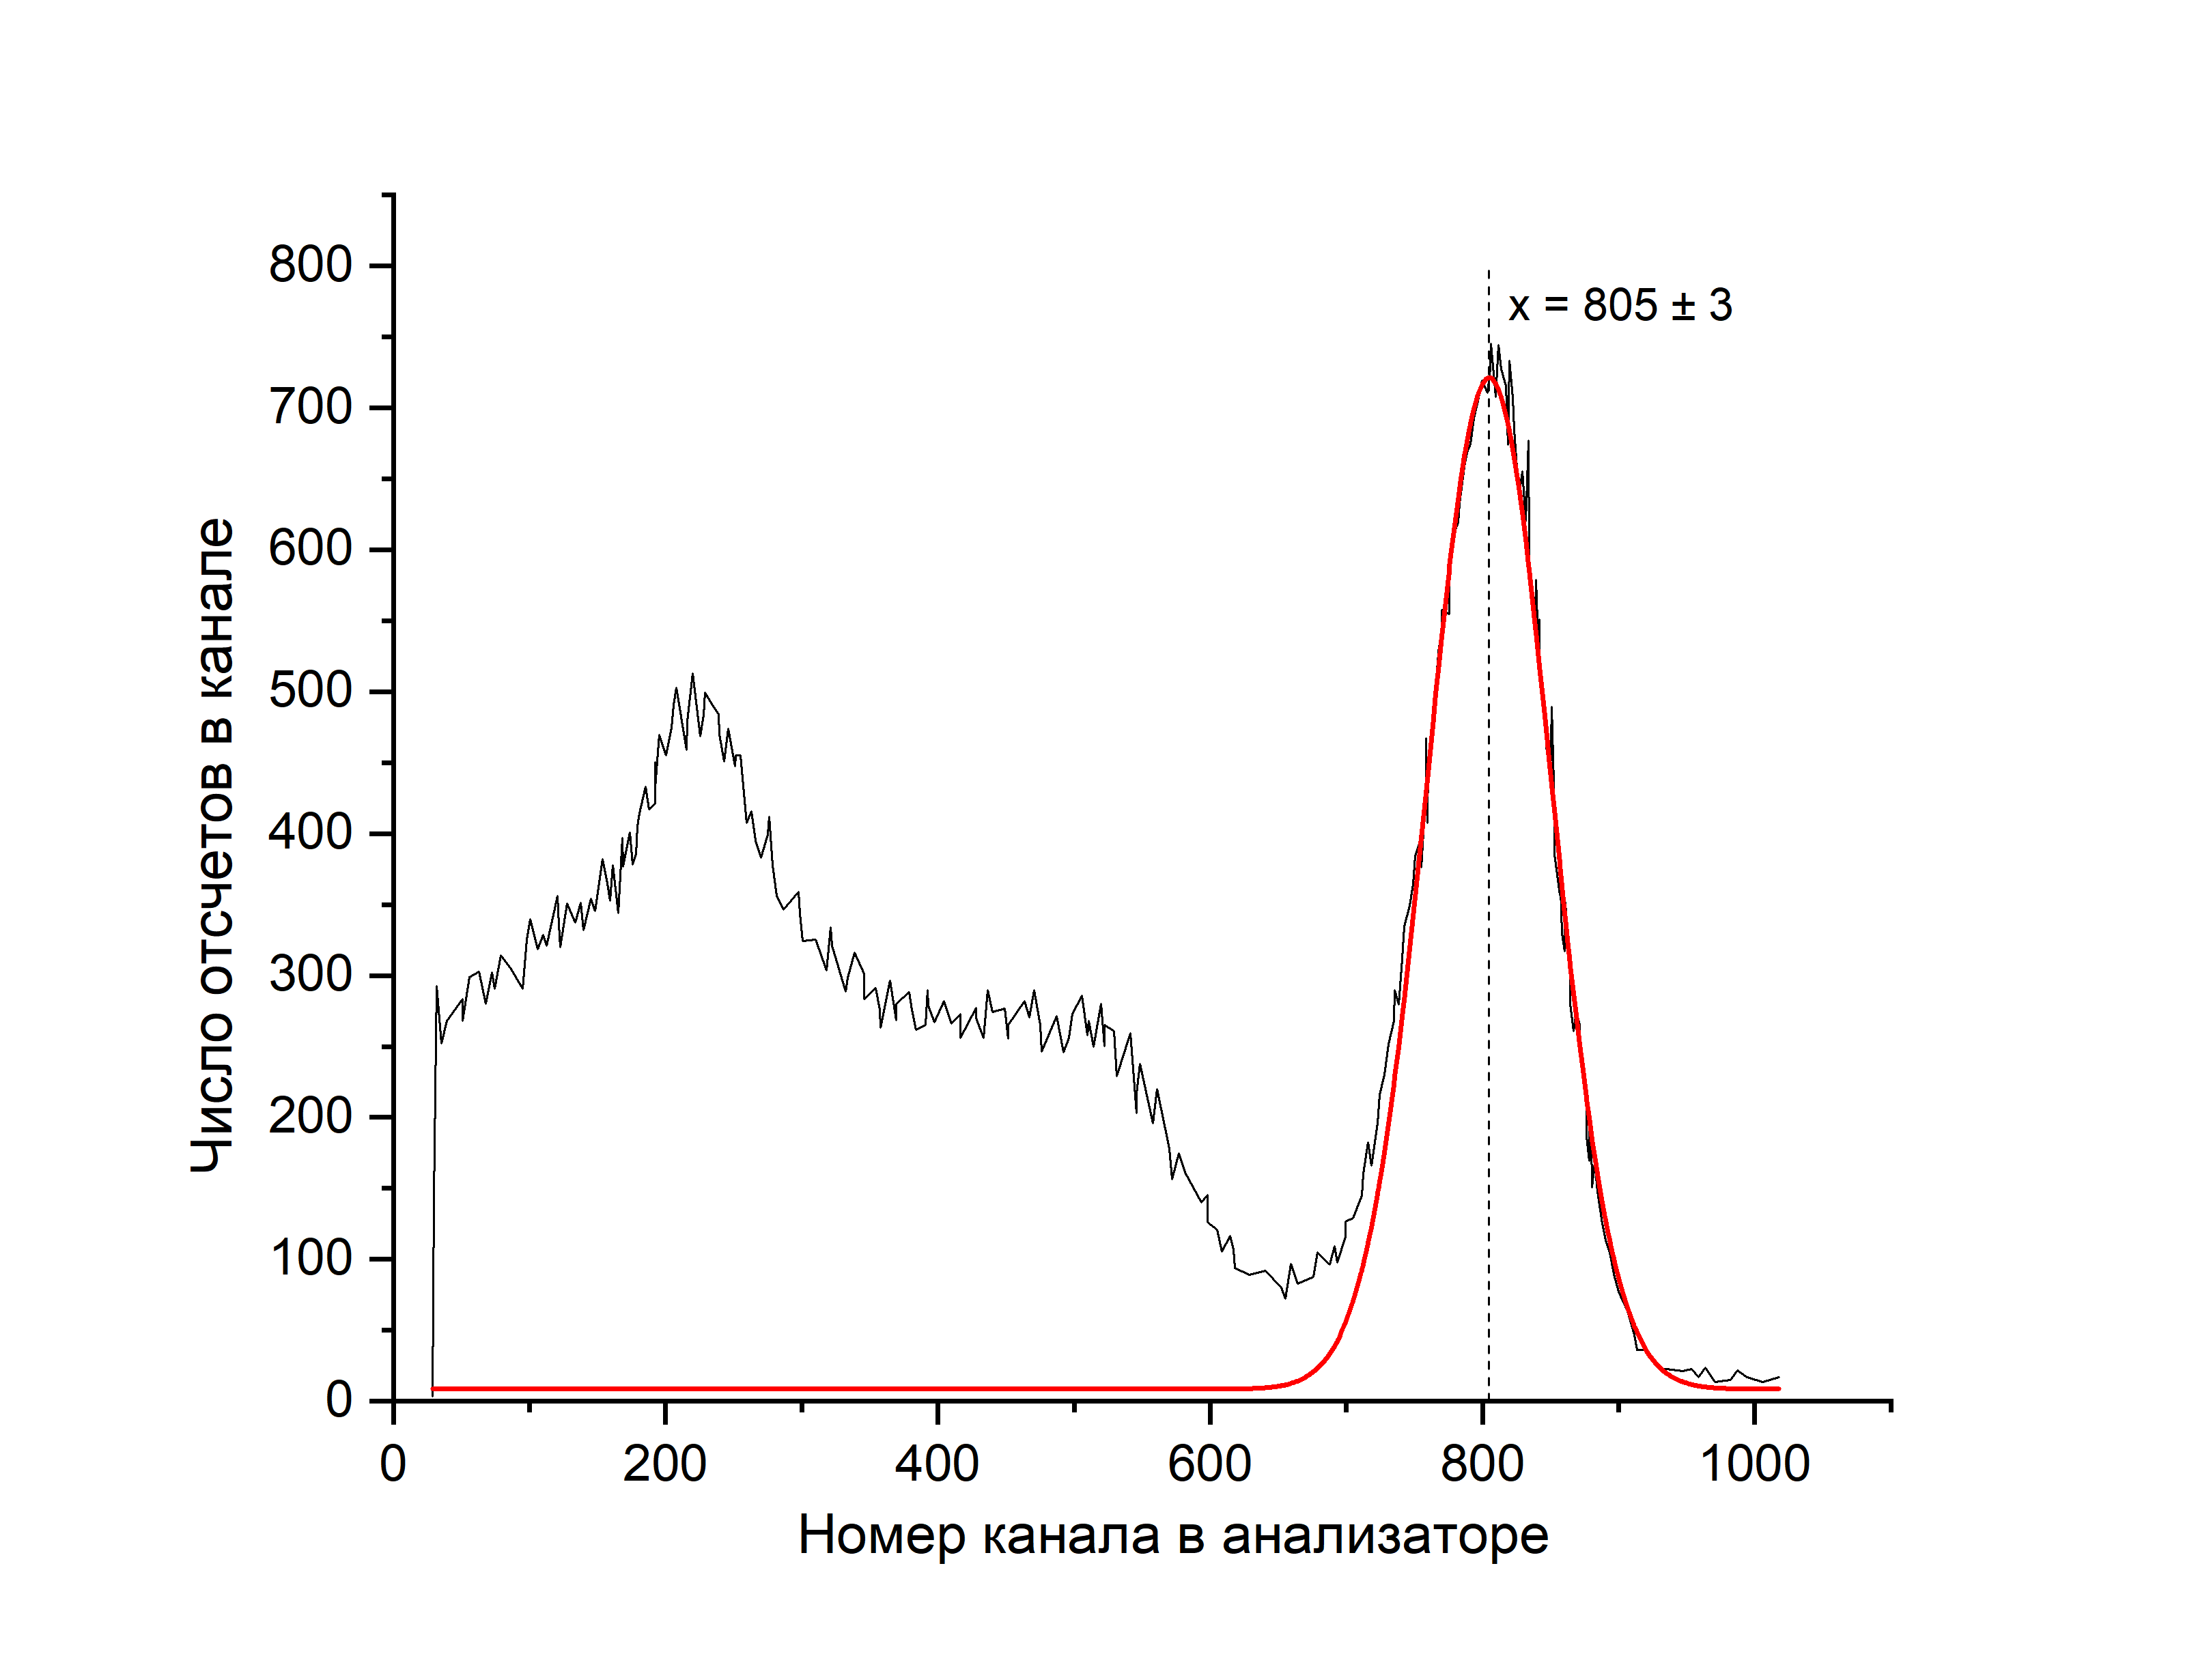
\includegraphics[scale=0.5]{оцифровка_0.png}
    \caption{\theta = 0 ^\circ}
\end{figure}

\begin{figure}[h!]
    \centering
    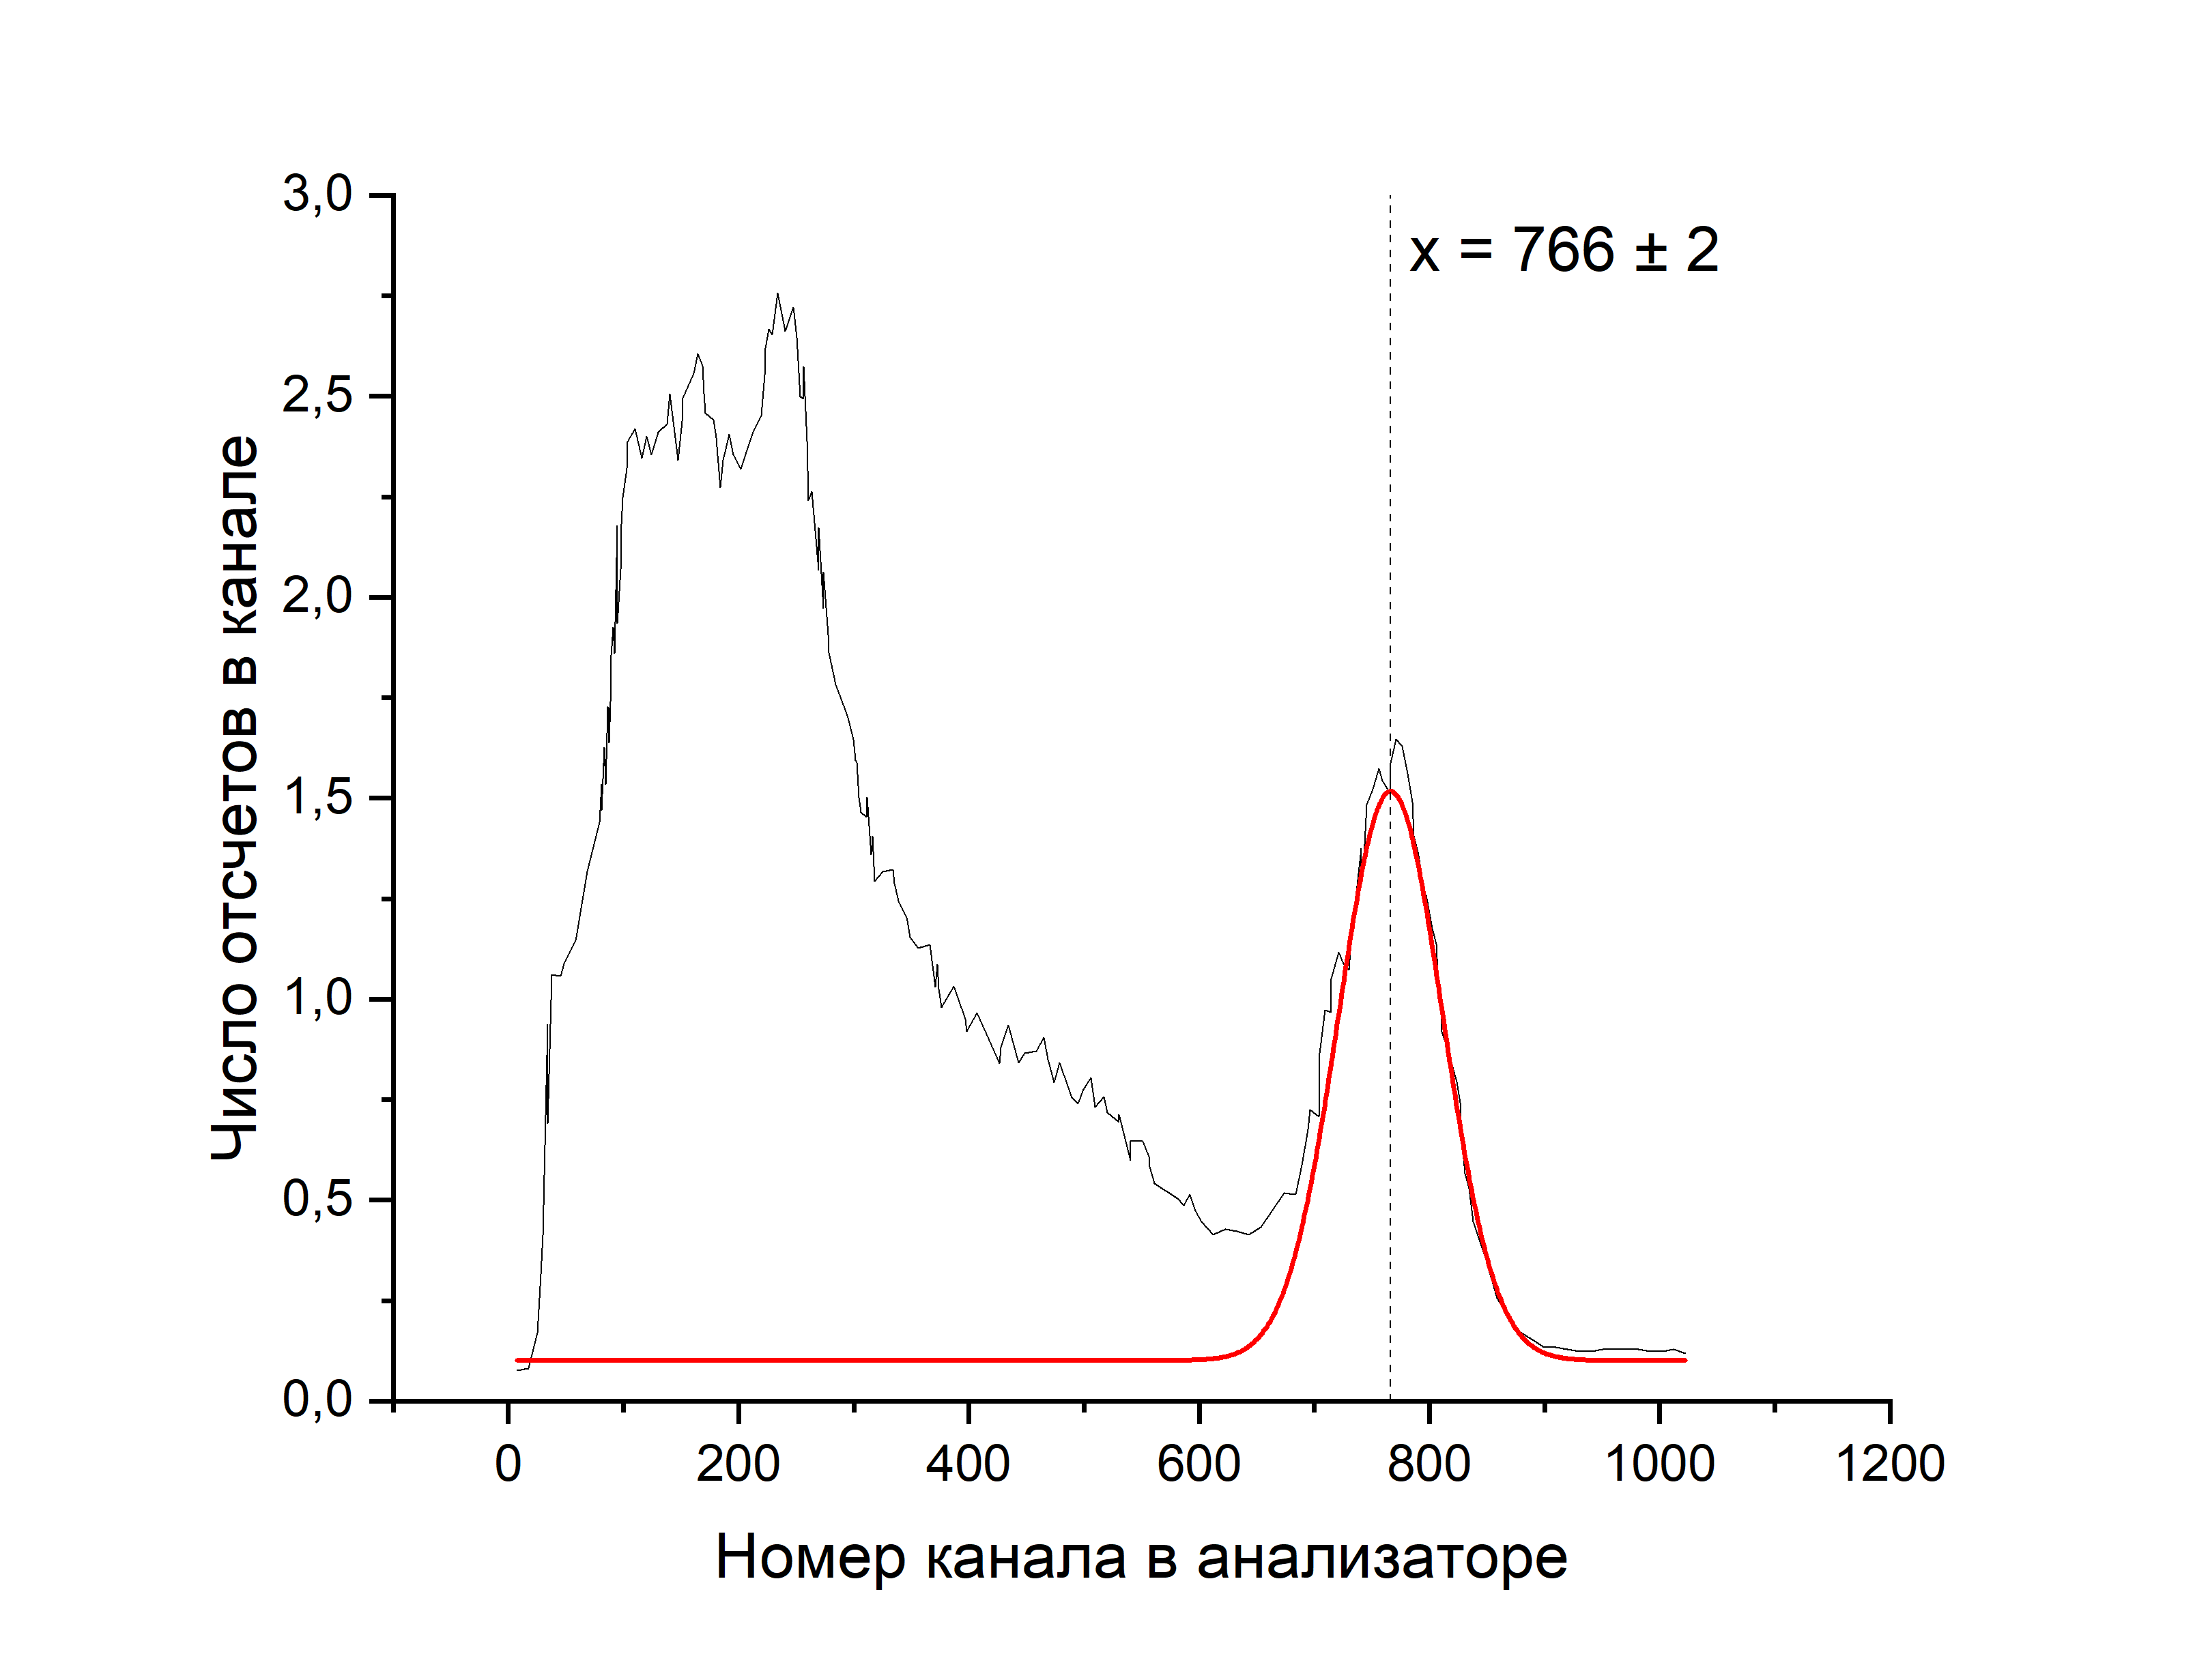
\includegraphics[scale=0.5]{оцифровка_20.png}
    \caption{\theta = 20 ^\circ}
\end{figure}

\begin{figure}[h!]
    \centering
    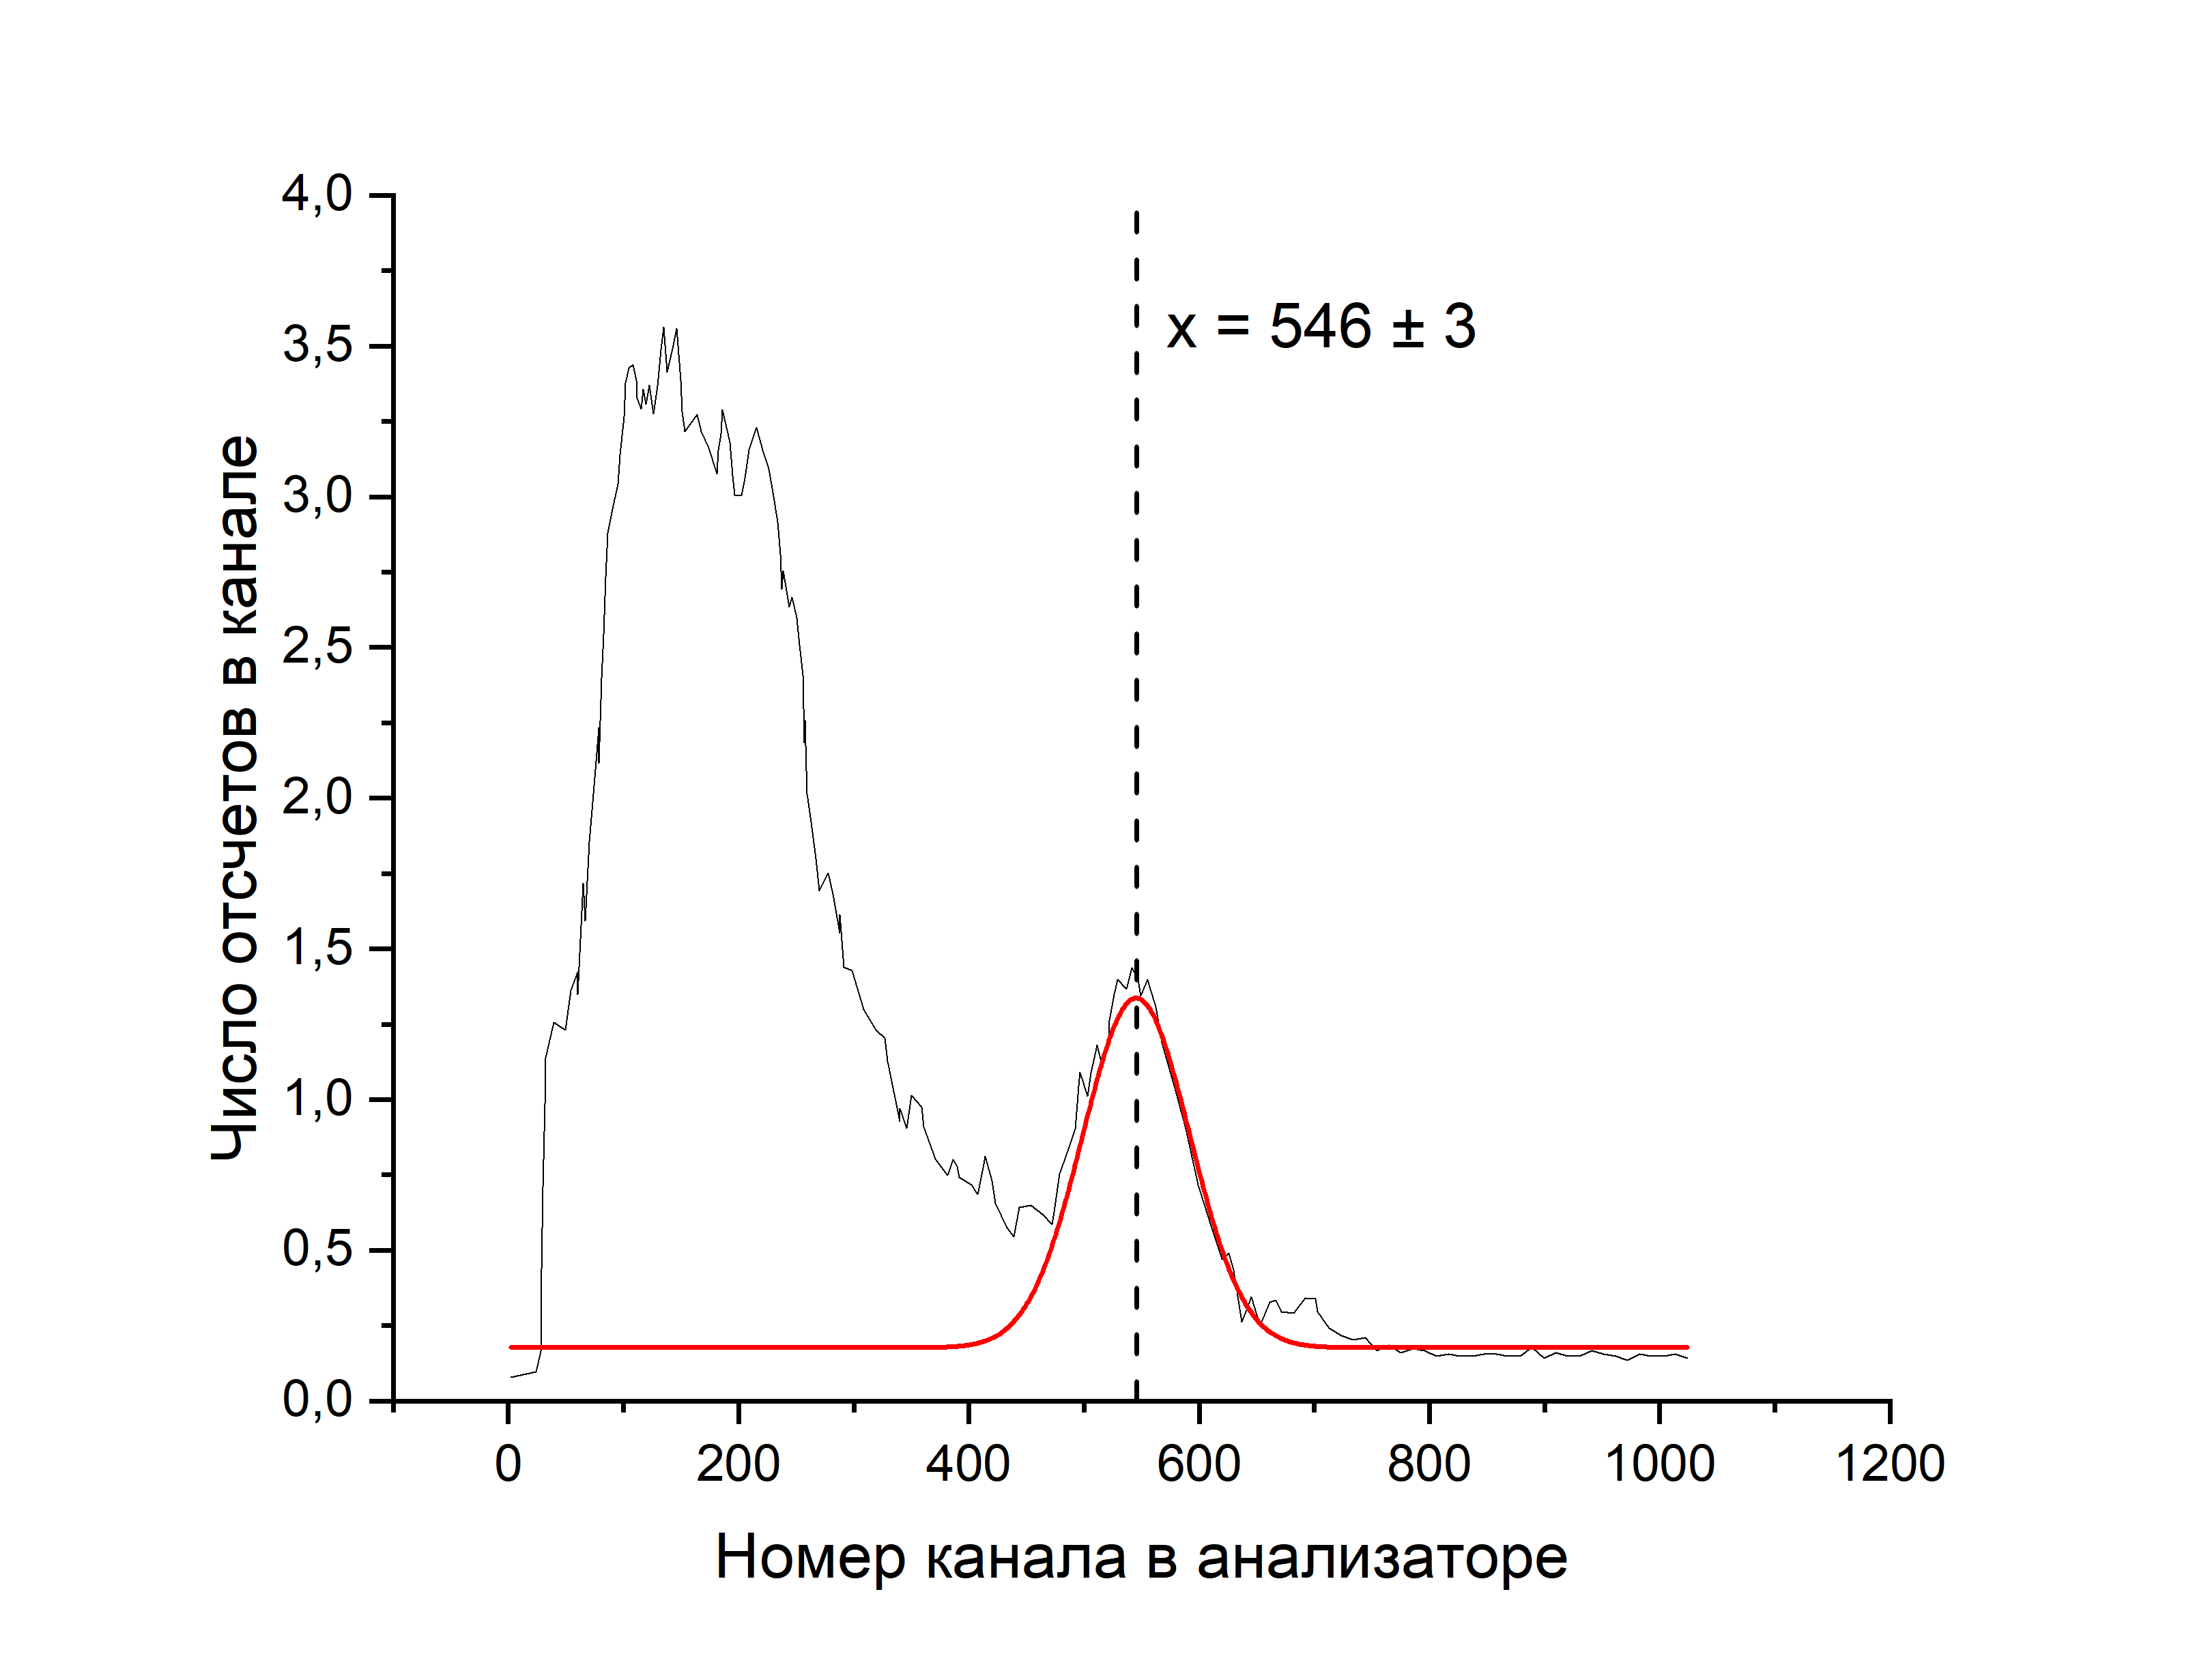
\includegraphics[scale=0.5]{оцифровка_50.png}
    \caption{\theta = 50 ^\circ}
\end{figure}

\begin{figure}[h!]
    \centering
    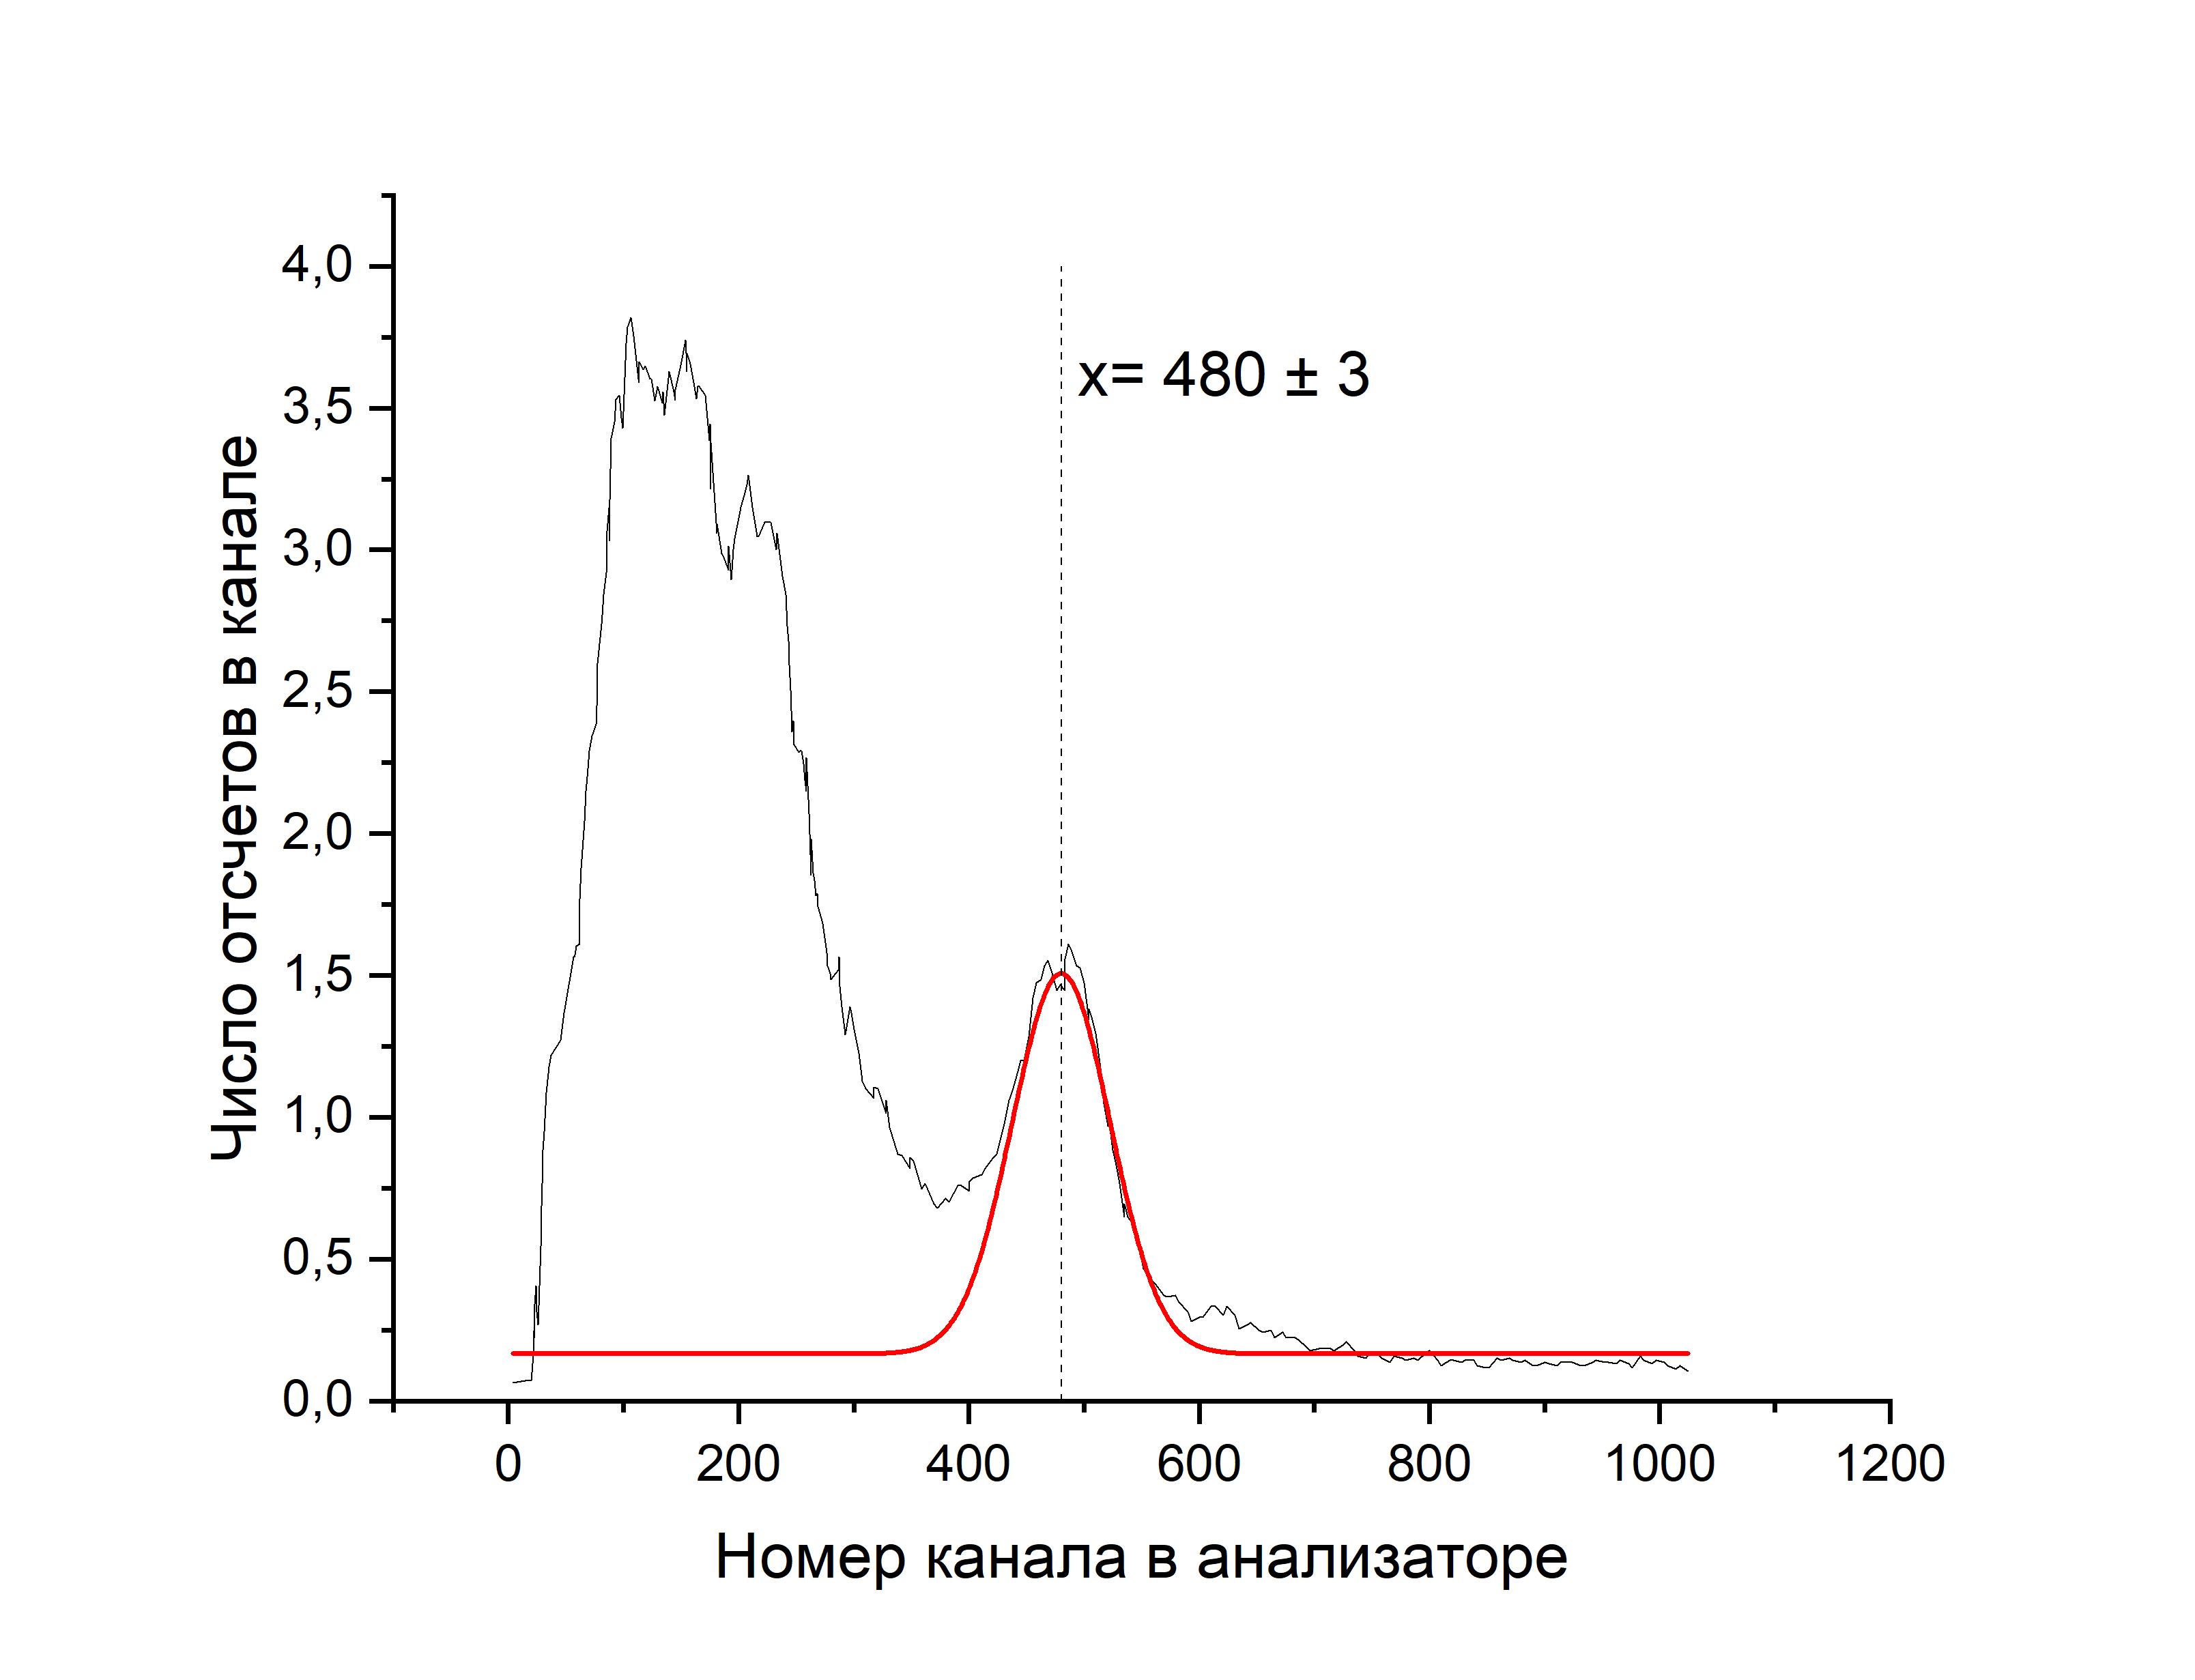
\includegraphics[scale=0.5]{оцифровка_60.png}
    \caption{\theta = 60 ^\circ}
\end{figure}

\begin{figure}[h!]
    \centering
    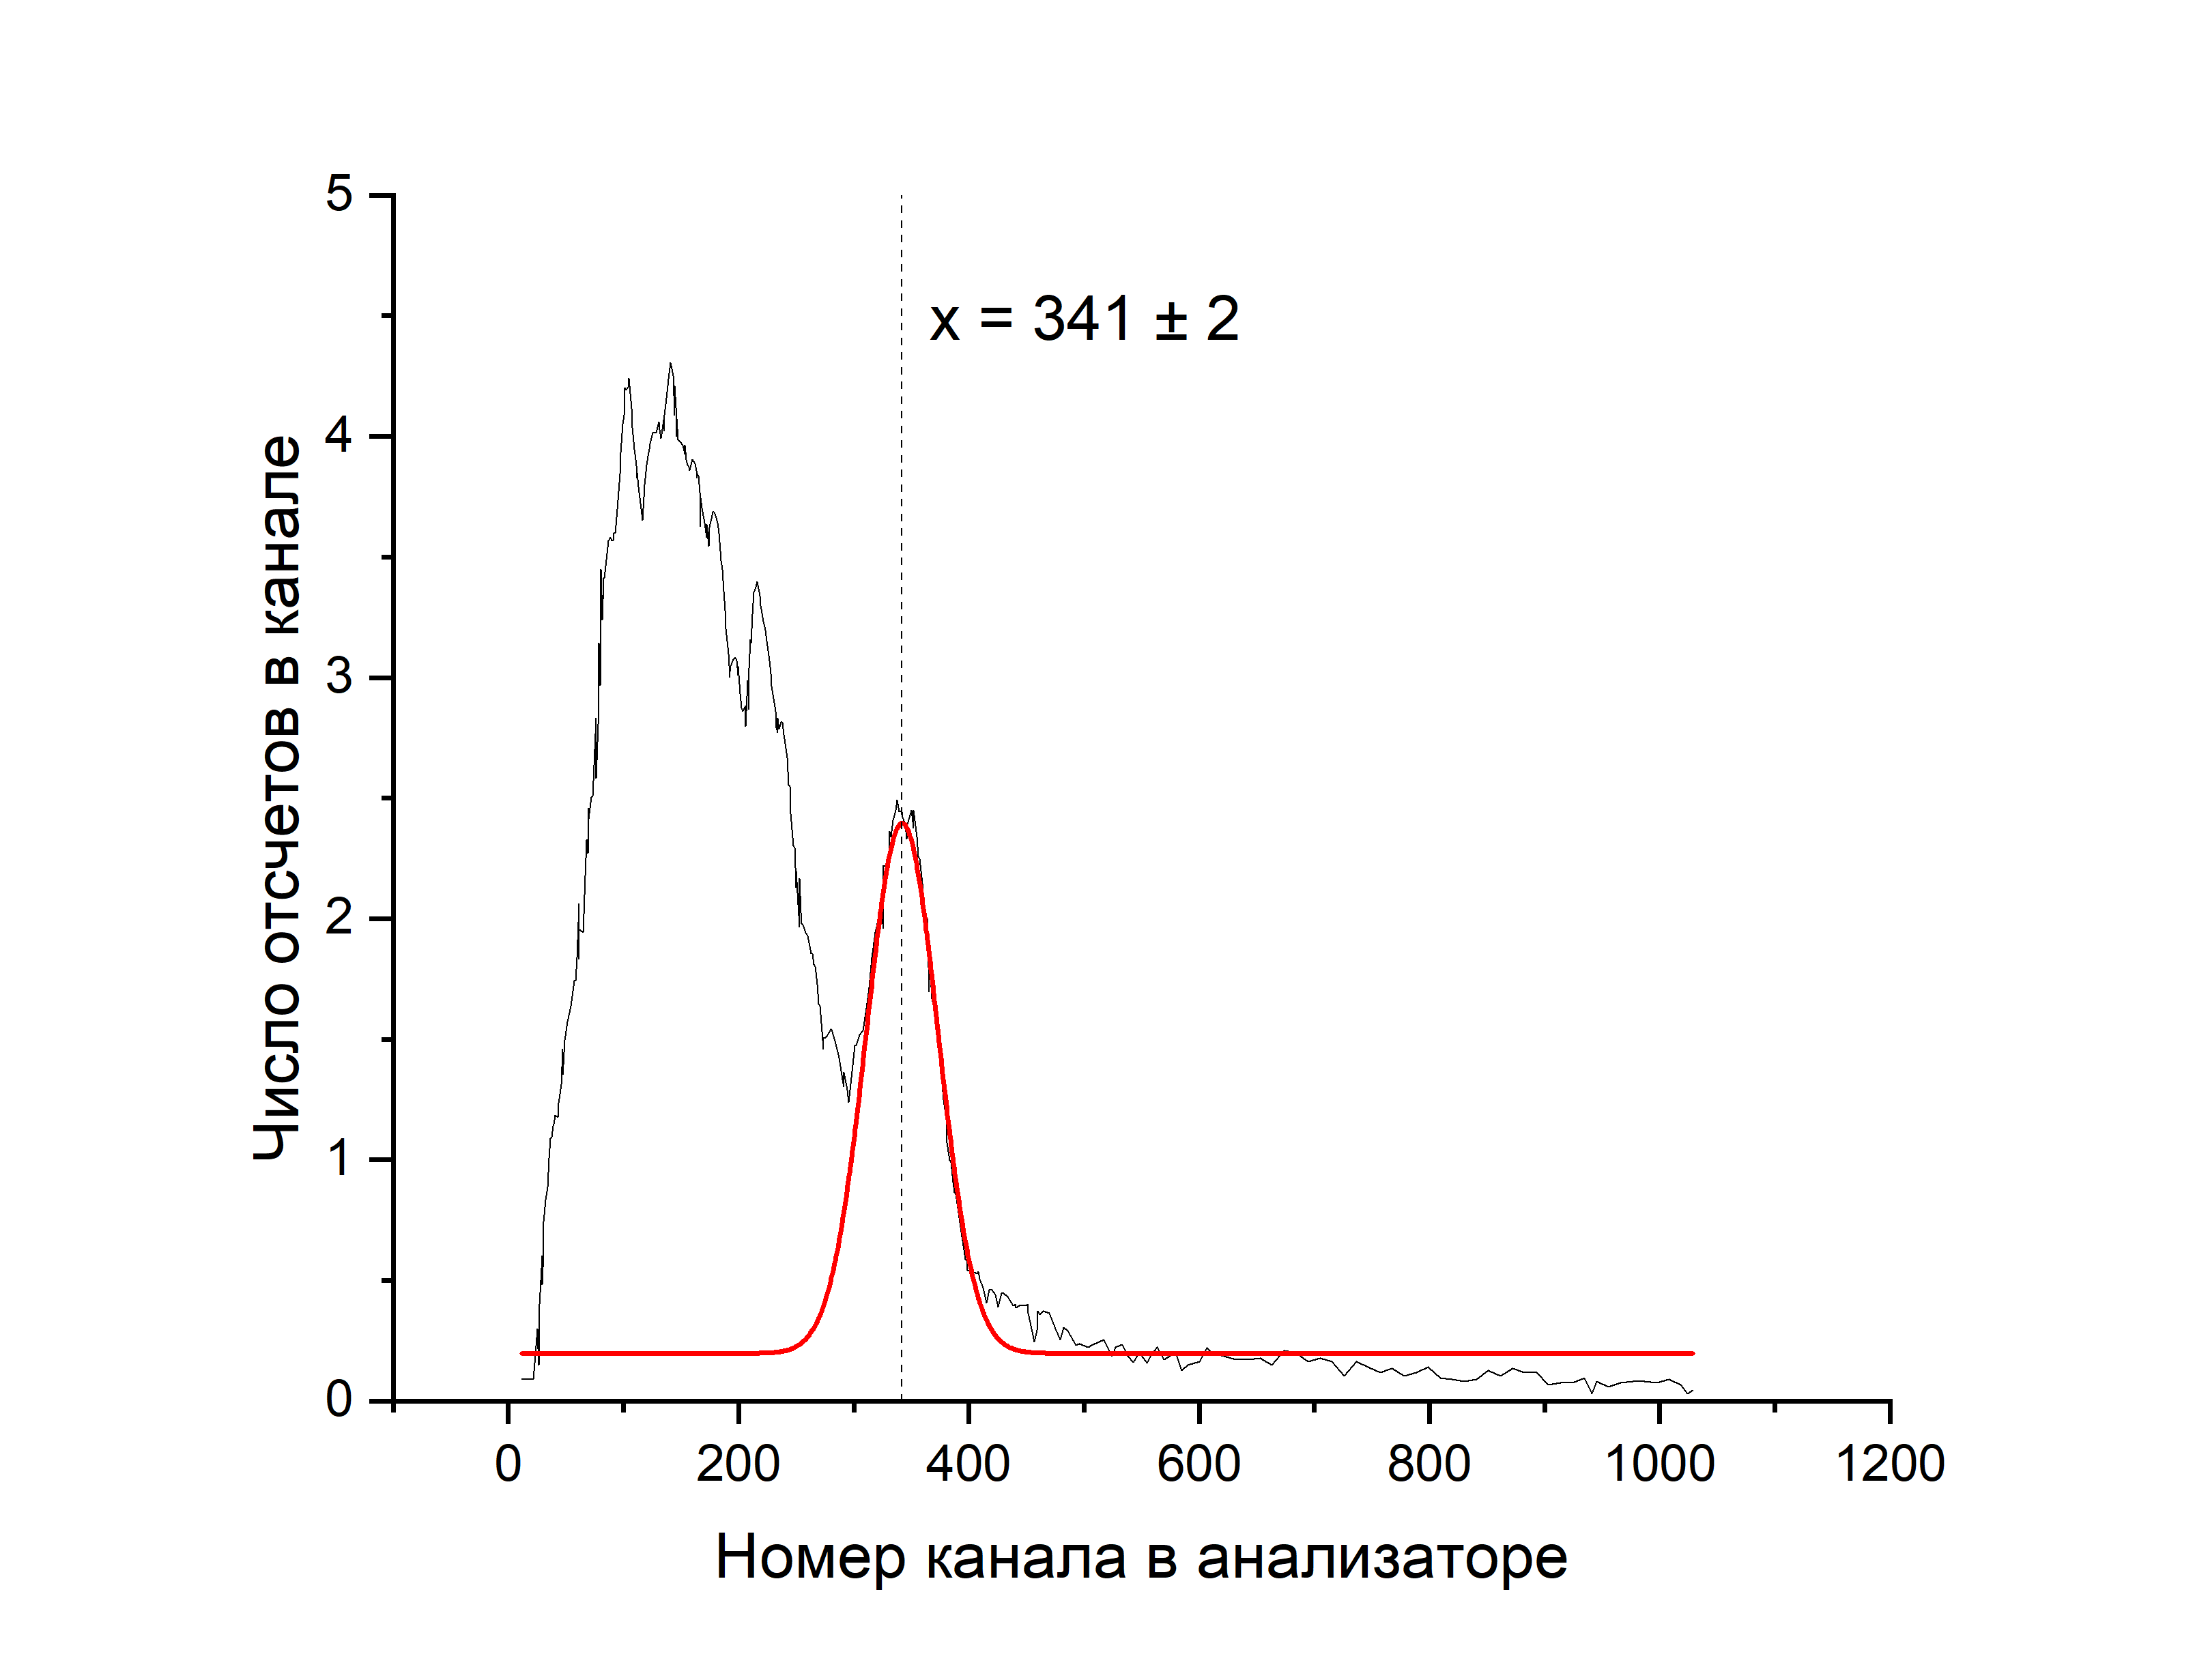
\includegraphics[scale=0.5]{оцифровка_90.png}
    \caption{\theta = 90 ^\circ}
\end{figure}

\end{document}